\section { 多级库存管理}

\subsection { 多级库存管理的内容}

    库存的最优化配置是企业重要的业务功能。低库存带来的制造、分销或零售运作上的优势表现为营运资本的永久性减少、更高的销售量和客户满意度。正如Forrester Research 在近期的一份报告上指出的那样,增强库存周转的能力是企业导致成功与失败的主要因素之一。

    管理库存是企业的艰巨任务,特别是那些在多个地方都拥有好几万种商品的企业。当这些商品处于企业分销网络的不同层级时,这种挑战就更为突出了。在这种多层级网络中,新产品出货后首先储存在地区或者中心机构中。这些中心机构是面对客户端的内部供应商。对于零售渠道和大型分销商和制造商而言,这是一种普遍的分销模式。比如,大型的医药批发商的分销网络包括一个地区性分销中心(RDC)和超过30 种的前向分销中心(DC)。另一种汽车零部件和设备的全国性零售商管理了超过2500 万库存单元(SKU),这些库存单元跨越了10 个DC 和超过900 家店。最后家具构件的全球制造商/分销商在将产成品运送到全世界15个当地DC 前,首先从位于工厂附近的欧洲DC 装货。然后由这15 个DC 服务终端的顾客。

    与单层网络相比,在多层级网络中管理库存都存在很多缺陷。缺陷之一是不能实现真正的网络库存优化,因为补货战略通常是应用于同一级的,而没有考虑对其他层级的冲击。当你仅仅处理一个单一层级时,通常缺乏对整个需求链上的库存使用状况的系统性看法。另一大缺陷是将上一层级的补货决策建立在华而不实的需求预测基础上。而这些缺陷能产生出各种相关的负结果,包括:

    \begin{enumerate}
        \item  网络以多余安全库存的形式保留了过多的库存;
        \item  即使网络中存在充足的库存,终端顾客服务缺陷仍然发生;
        \item  当层级之间的服务超过可接受的范围时,面对客户的供应点发生令人不快的存货短缺;
        \item  外部供应商提供不可靠的业绩信息,因为他们接收了令人不满意的需求指示;
        \item  目光短浅的内部产品配置决策是非常有限的。
    \end{enumerate}

\textbf { 多级分销网络}

    多层级分销网络(如,一个网络包括一个中心仓库和下游多个客户端供应点)中管理库存的复杂性在不断增加。所有这些分销点是在一个单一企业的内部控制之下。在单个层级状态,尽管你不需要在供应商和终端客户之间的仓库或者DC 进行补货,但是你仍然需要解决供应商和DC 之间的其他分销点的补货问题。多级库存管理的目的是在最小网络库存的情况下(而这些库存是分散在各个不同的层级中的),实现令终端顾客满意的服务。

\textbf { 在单层级网络中的库存管理}

    在研究一个以上层级中进行库存管理的困难之前,让我们首先回顾一下单层级网络中存在的问题。在这个环境中,分销网络是供应商 DC  顾客。表 \ref{tab:dcsku} 描述了位于DC 附近的SKU库存驱动因素。

    在这个单层级状态中,订货至交货的前置时间主要是停留在DC 和它的外部供应商。企业的订单供应策略取决于它的内部成本因素——诸如那些与处理和运输库存相关的成本——以及外部供应商的订单限制和折扣。由于这个原因,补货数量既取决于内部因素,又取决于外部因素。

    \begin{table}[bcth]
        %\footnotesize
        \caption{位于DC 的SKU 的库存驱动因素} \label{tab:dcsku}
        \vskip 1em
        \begin{tabular}{|c|c|}
            \hline
             库存 & 描述 \\ \hline
             需求 & 产品流出 DC 的比例 \\ \hline
             需求变化 & 不同时期产品流出的波动 \\ \hline
             前置时间 & 订单和满足需求的新产品交货的预期时间间隔 \\ \hline
             前置时间的变化 & 不同订单前置时间的波动 \\ \hline
             补货周转率 & DC 检查存货是否需要下新订单的周期 \\ \hline
             订单供应战略 & DC的时间供应目标,它取决于装存货、处理、运输存货和购买成本之间的经济性比较 \\ \hline
             库存位置 & DC可获得的库存,需要考虑的在手库存、已下订单的数量、未交清订货、关键库存 \\ \hline
        \end{tabular}
    \end{table}

\textbf { 多层级网络中的库存管理}

    现在考虑同样的产品在多层级网络中的情况,这里的多层级网络是指在供应商和DC 之间还包括一个RDC。相同的库存驱动因素如前所述。然而,一些重要的问题出现了:

    \begin{enumerate}
        \item  预测 RDC 需求的正确方法是什么,如何预测这个需求?
        \item  你怎样预测 RDC 需求出现的差异?
        \item  来自 RDC 至供应商的订单更大的趋势怎样影响RDC SKU 的订单供应战略?
        \item  在 RDC 和它的“顾客”之间的最佳服务水平目标是什么?哪一个是DC 的?
        \item  你怎样将单个 DC 的库存定位纳入RDC 补货决策之中?
        \item  RDC 中的库存驱动因素如补货周转率和服务水平目标怎样影响DC 层级的服务库存和服务水平?
        \item  当面临着 RDC 中有限的供应状况时,你怎样将产品分配至DC?
    \end{enumerate}

    因为 RDC 同样为SKU 保持库存,而DC 又和内部供应商之间存在着关系,所以在进行DC 补货决策也必须解决一些新问题:

    \begin{enumerate}
        \item  由 RDC 施加的订单限制怎样影响DC 的订单供应战略?
        \item  不同的 DC 补货周转率和替补订单供应战略怎样影响RDC?你怎样将RDC 服务水平目标纳入DC 补货战略之中?
        \item  为了获得向终端客户承诺的目标服务水平,当 RDC 对终端客户而言,像后备资源那样可获得时,DC 应该确立相同的服务水平目标吗?
        \item  你怎样才能在迅速的订单流程中使用 RDC?
        \item  外部供应商的前置时间和前置时间的差异在 DC 的补货战略中仍然扮演着重要的角色吗?
    \end{enumerate}

    \begin{figure}[bcth]
        \begin{center}
            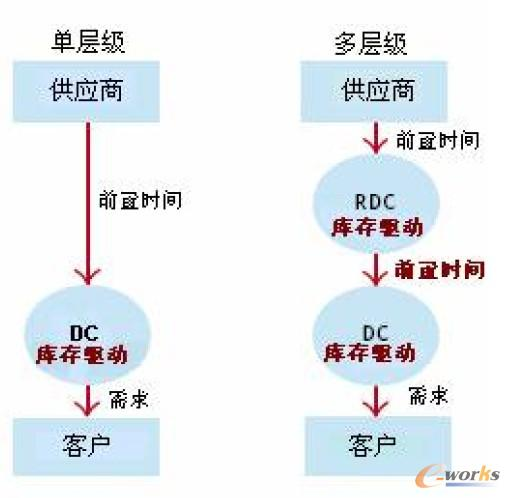
\includegraphics[scale=.6] {ml-info.jpg}
            \caption {库存驱动} \label {fig:mlinfo}
        \end{center}
    \end{figure}

    图 \ref{fig:mlinfo} 阐述了库存驱动因素怎样在两个层级中联系起来。循环节点代表了企业控制下的分销中心。标有“DC”的节点代表存储相同产品的所有DC。用红色标出的库存驱动因素是企业可以控制的。也就是说,补货周转率、订单供应战略和服务水平目标是补货控制变量,一个决策制定者能够影响装载的库存数量和提供给下端客户的服务水平。在单层级案例中决定控制变量的方法是众所周知的,但是你怎样才能在多层级案例中设置控制变量呢?今天,企业主要使用以下两种方法:

    \begin{enumerate}
        \item  将单层级方法应用到网络中的每个层级中。
        \item  使用配送需要计划(DRP)方法或者它的改进方法。
    \end{enumerate}
